\chapter{Density Gradient Fields of the Defocused Pressure Ratio Sweep}
\label{Appendix: aerospike defocused NPR sweep}

\par Figure \ref{fig: aerospike density gradients NPR sweep} presents the density gradient fields of points 8 to 11, which imaged the nozzle pressure ratios of 8, 10, 12 and 14 with the camera focused inside the test section. The same four conditions were also acquired with the in-focus plane 55 mm in front of the model, as points 4 to 7 of Table \ref{tab: aerospike test matrix}, and the density gradients that follow from them are displayed in Figure \ref{fig: aerospike density gradients NPR sweep defocused}. These points were used in Section \ref{subsection: Aerospike S Ratio} only through their maximum displacements, which fed the ratio method that provided the sensitivity of the in-focus points, so their fields were not shown in the main text and are reproduced here for completeness. As the focus of these configurations lies in front of the test section, the geometric model holds and the gradients were obtained directly with the effective lever arm $l_{eff} = l + G + W/2 = 160$ mm of the test matrix, assuming a planar flow as before.

\par Comparing the four pairs with those of Figure \ref{fig: aerospike density gradients NPR sweep}, the defocused points resolve the same structures and follow the same trends. The initial compression wave that leaves the ramp extends further downstream as the nozzle pressure ratio increases, the reflections shift to the right and the expansion fan at the tip turns more sharply down, which is the behavior discussed in Section \ref{subsection: Aerospike Flow Structure}. The agreement is also quantitative, since the peaks of points 4 and 8, which imaged the same flow condition, remained within 17.3\% of each other and below 10\% when the 100 highest values were averaged, as presented in Table \ref{tab: aerospike gradient peaks freestream}. Nevertheless, the fields of these points show a grainier texture than their in-focus counterparts, which follows from the increased blur. Propagated through the planar relation, its median ranges from 0.0014 to 0.0021 kg m$^{-3}$ mm$^{-1}$ across points 4 to 7, against 0.0007 to 0.0012 kg m$^{-3}$ mm$^{-1}$ across points 8 to 11, so roughly twice as much.

\par Another observation concerns point 7, the condition at which the flow of point 11 changed dramatically. The standing shock that forms at the edge of the ramp in Figure \ref{fig: aerospike density gradient point 11} is absent from Figure \ref{fig: aerospike density gradient point 7}, whose field continues the progression of points 4 to 6 instead. Therefore, the defocused sweep supports the interpretation given in Section \ref{subsection: Aerospike Flow Structure}, that point 11 was probably captured at a larger nozzle pressure ratio than point 7 and that the shock formed only in the former.

\begin{figure}[htbp]
    \centering
    \begin{subfigure}[b]{\textwidth}
        \centering
        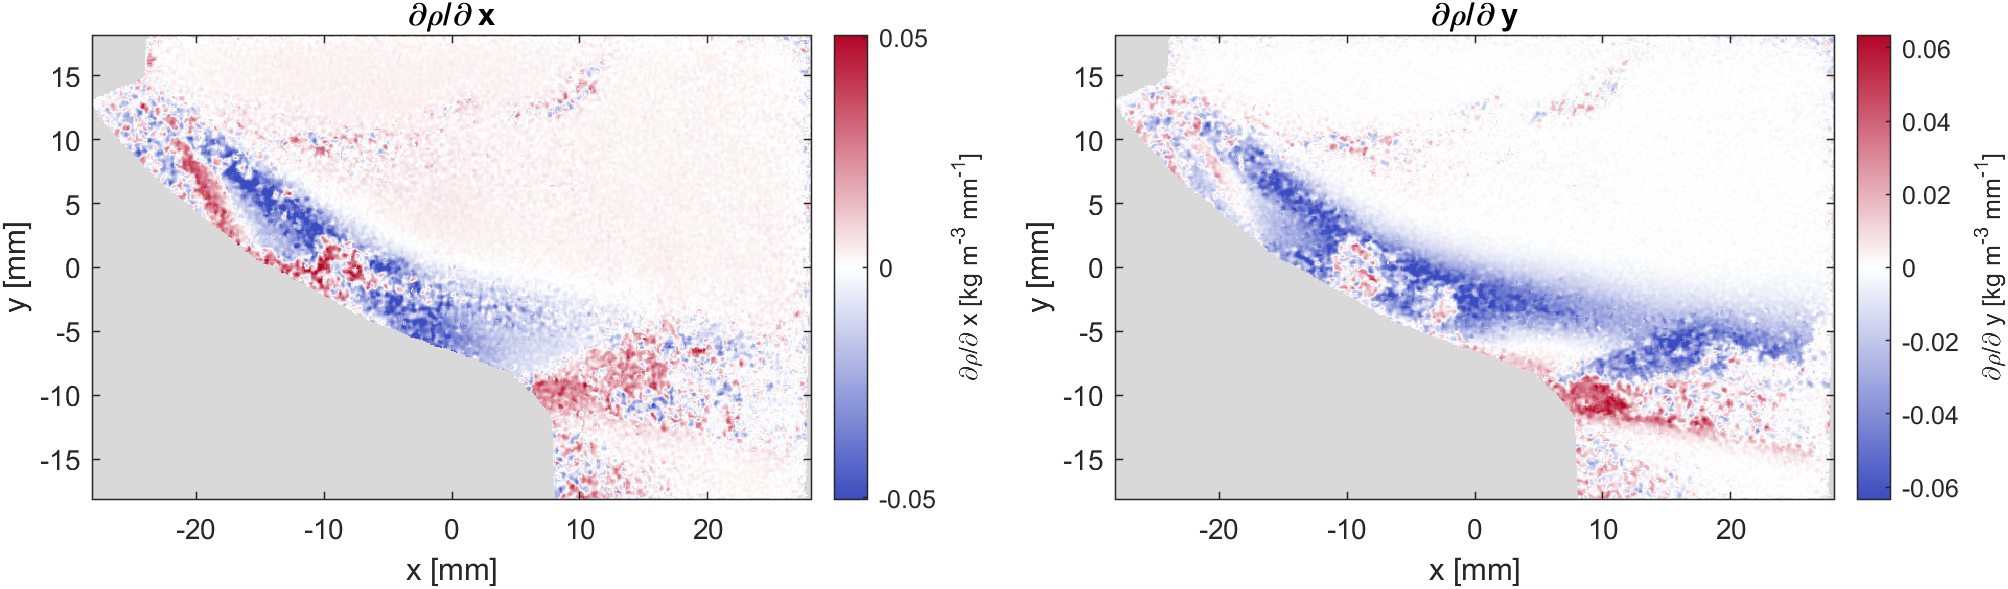
\includegraphics[width=0.97\textwidth]{figures/aerospike density gradient point 4.png}
        \caption{Point 4, $NPR = 8$}
        \label{fig: aerospike density gradient point 4}
    \end{subfigure}

    \begin{subfigure}[b]{\textwidth}
        \centering
        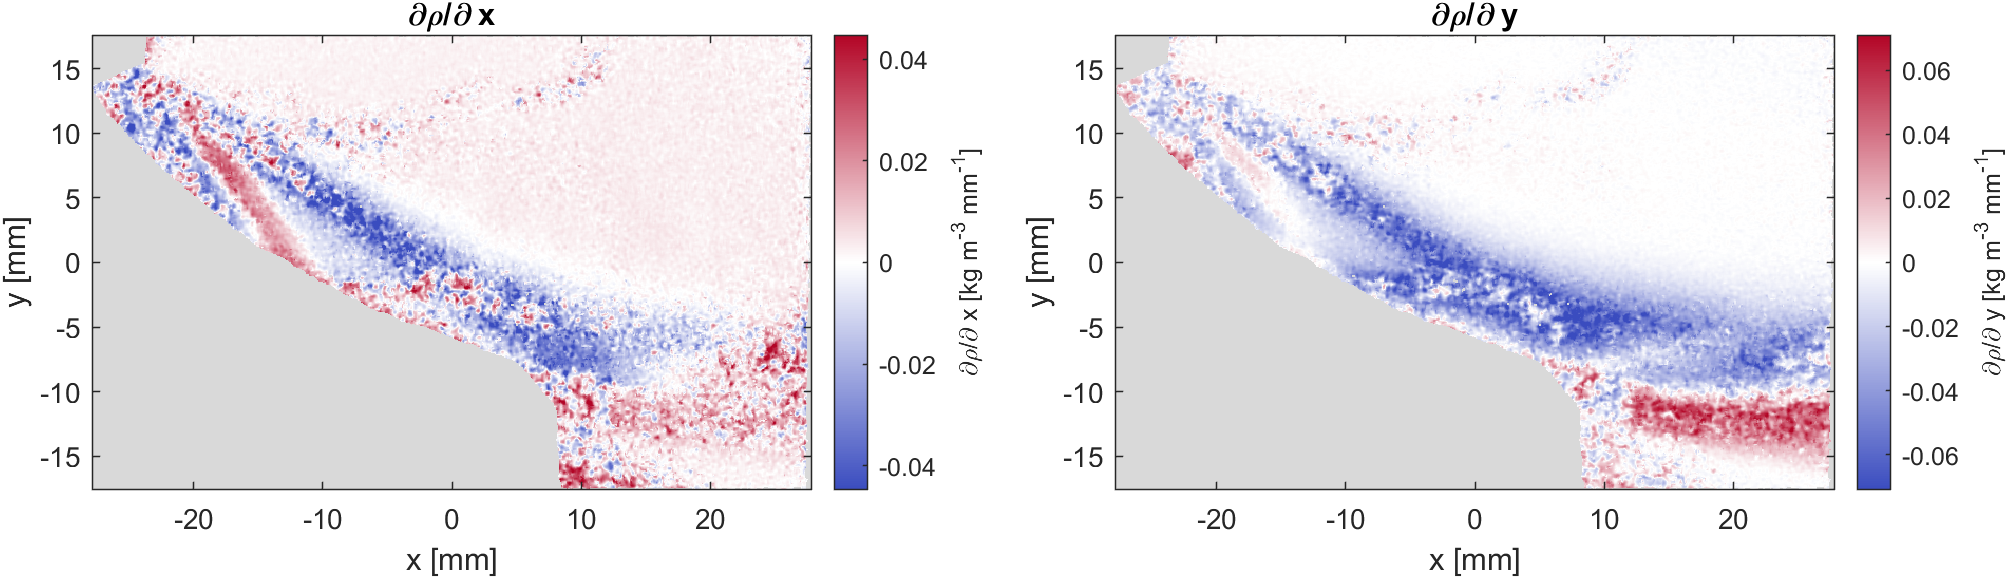
\includegraphics[width=0.97\textwidth]{figures/aerospike density gradient point 5.png}
        \caption{Point 5, $NPR = 10$}
        \label{fig: aerospike density gradient point 5}
    \end{subfigure}

    \begin{subfigure}[b]{\textwidth}
        \centering
        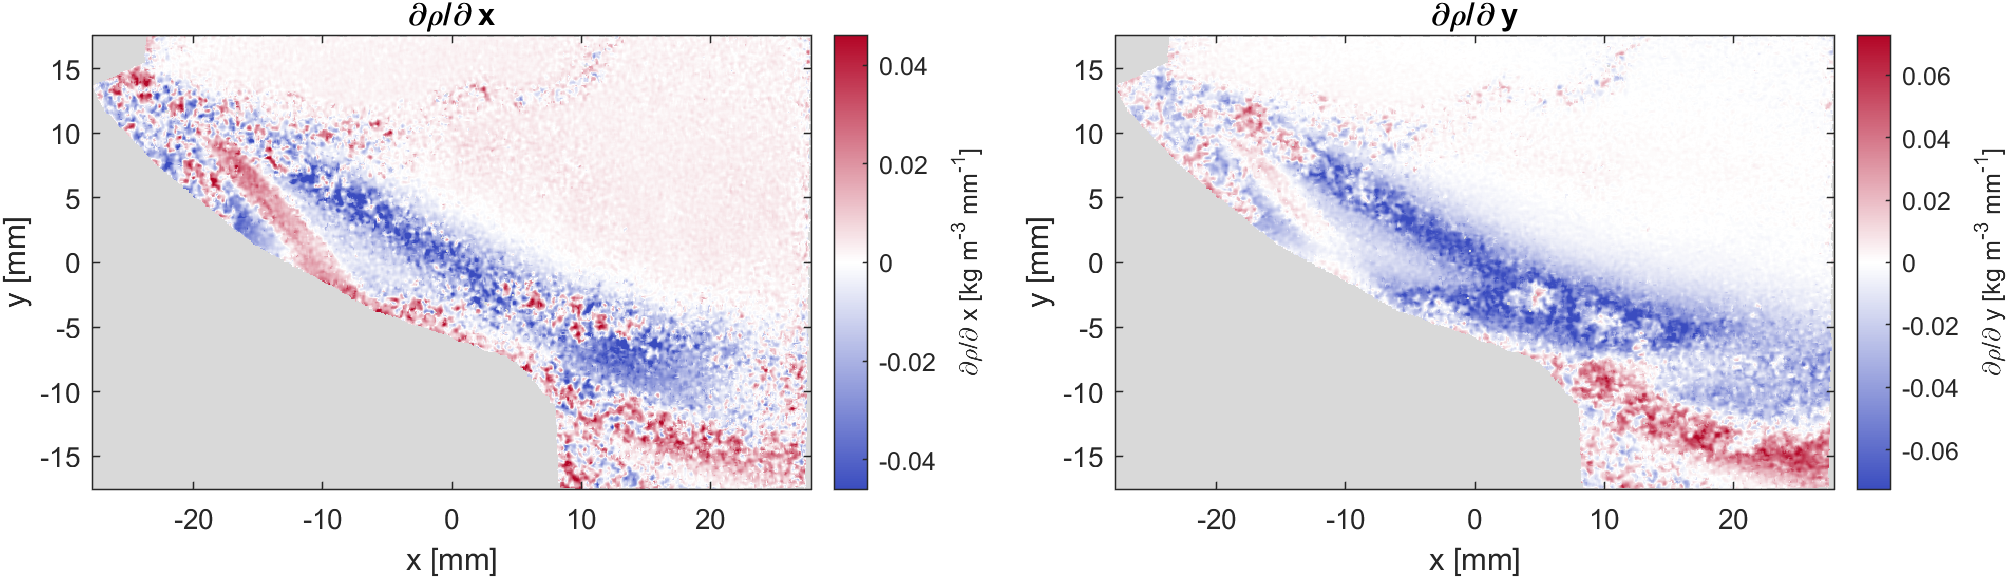
\includegraphics[width=0.97\textwidth]{figures/aerospike density gradient point 6.png}
        \caption{Point 6, $NPR = 12$}
        \label{fig: aerospike density gradient point 6}
    \end{subfigure}

    \begin{subfigure}[b]{\textwidth}
        \centering
        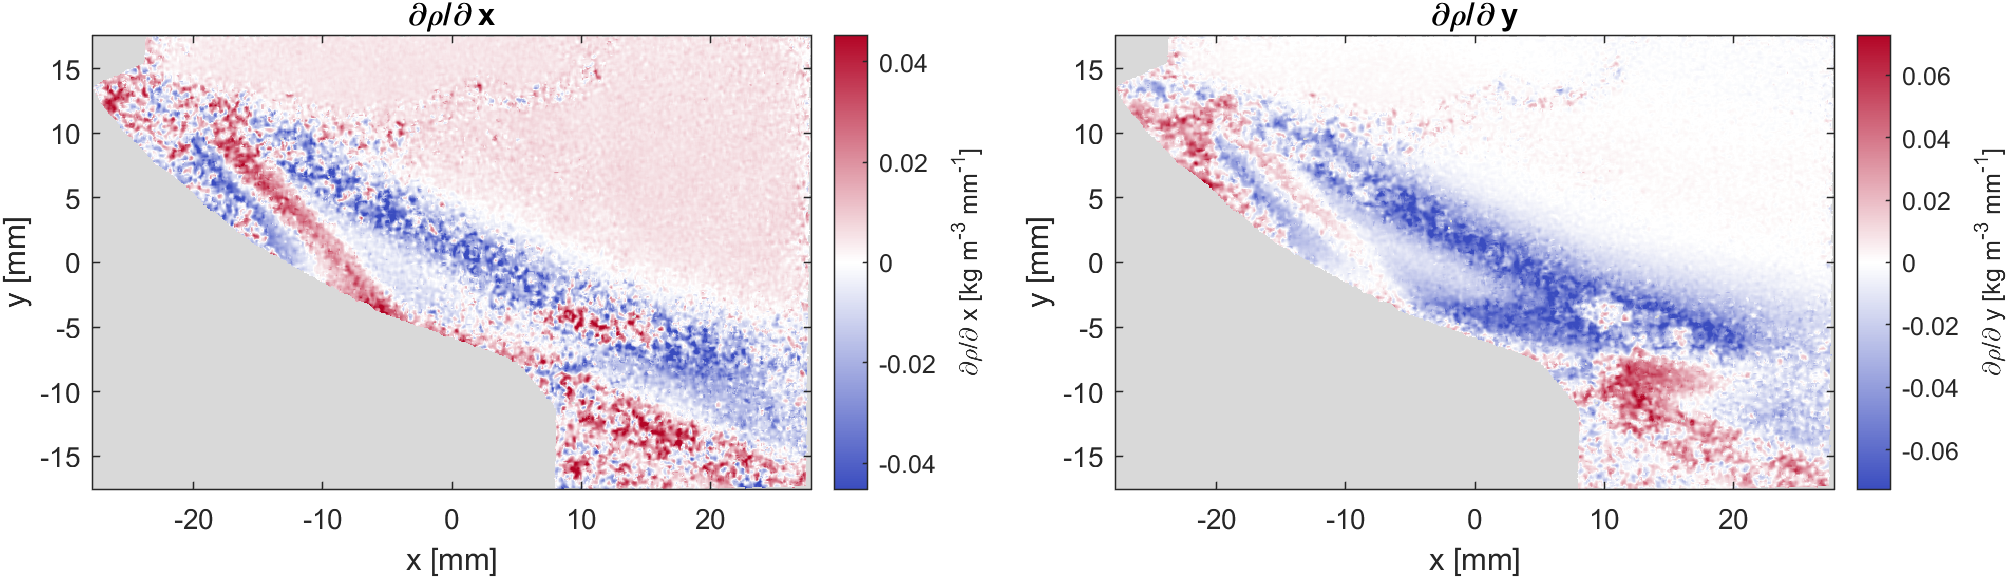
\includegraphics[width=0.97\textwidth]{figures/aerospike density gradient point 7.png}
        \caption{Point 7, $NPR = 14$}
        \label{fig: aerospike density gradient point 7}
    \end{subfigure}
    \caption[Density gradient fields of the defocused $NPR$ sweep]{Density gradient fields of points 4 to 7, obtained assuming a planar flow with the effective lever arm $l_{eff} = 160$ mm of Table \ref{tab: aerospike test matrix}. Each row displays the component in the $x$ direction on the left and the component in the $y$ direction on the right, for one nozzle pressure ratio. Each field uses its own color scale and masked regions are shown in grey}
    \label{fig: aerospike density gradients NPR sweep defocused}
\end{figure}
